\documentclass{book}
\usepackage{graphicx} %LaTeX package to import graphics
\graphicspath{{img/}} %configuring the graphicx package

\begin{document}

\chapter{Introduction}

\section*{Methodologie de Travail}

Pour la méthodologie de travail que l'on suivre dans ce projet de fin d'année, nous orientons vers le modéle itérative incrémental plus précisement nous utilisons l'agilité, pour avancer dans ce projet en gardant toujours un executable fonctionnelle et validés jusqu'a au bout du projet.
Les raisons que nous attire a choisir ce type de modéle sont comme mentionnée dans [1]
\begin{itemize}
  \item Time-to-Market
\\Accélérer la mise à disposition de nouveaux produits sur leur marché est au cœur des méthodes agiles car l’ensemble des rituels imposent un décloisonnement des métiers, plus de collaboration, plus de transparence entre les relations clients/fournisseurs, plus de réactivité.
  \item Collaboration et engagement.
  \\L’agilité, c’est aussi des interactions constantes car le client est impliqué à chaque étape du projet. Le client est littéralement intégré au projet, ce qui permet aux équipes techniques de gagner en compréhension de ses enjeux et de ses attentes, c’est une boucle vertueuse. Fini le fameux effet tunnel. Les équipes sont davantage responsabilisées, polyvalentes et s’organisent mieux entre elles. On constate également une meilleure implication et motivation des équipes sur toute la durée du projet car il est très satisfaisant, pour toutes les parties prenantes, de livrer régulièrement un produit fonctionnel.
  \item Transparence totale
  \\L’agilité repose sur une communication transparente avec le client sur l’avancée du projet. Il est impliqué dans la priorisation des éléments et autres fonctionnalités à livrer jusqu’à la planification des itérations en passant par les tests fonctionnels. Par contre, cela sous-entend que votre client est bel et bien prêt à s’impliquer personnellement dans le projet et donc, dans une certaine mesure, à en partager les risques et en supporter les responsabilités.
  \item Qualité logicielle
  Dans la méthodologie Agile, des tests réguliers sont effectués à chaque sprint, ce qui permet de vérifier que la qualité est bien aux attendus et que le produit fonctionne à ce stade du développement… et de redresser le cas échéant. Cela permet plus de flexibilité lors de nouvelles modifications et de renforcer la vigilance en cas d’imprévus. Au final, l’agilité offre plus de réactivité en cas de problèmes car c’est encore "frais" ! Pas étonnant que sur ces deux dernières années, le nombre de "testeurs agiles" ait été multiplié par deux chez Harington, cela illustre à quel point les développements agiles nécessitent une très grande rigueur pour livrer un produit fiable et fidèle aux attendus métiers. On constate également que la qualité des livrables augmente ! Le code est plus facile à maintenir et il y a de moins en moins de défauts critiques lors de la mise en production.
  \item Le droit de changer d’avis
  \\ Dans l’agilité, contrairement aux méthodes traditionnelles (en cascade ou cycle en V), le changement est bienvenu et l’adaptation est la règle ! Les clients peuvent changer d’avis, faire évoluer leurs besoins et les équipes techniques peuvent aussi faire évoluer leurs choix technologiques. À tout moment, on peut arrêter le projet si on considère être dans une impasse. Le plus important est la stabilité des équipes qui gèrent le projet car elles s’engagent à délivrer un ensemble de fonctionnalités convenues ensemble, à chaque sprint. A chaque itération, les équipes accumulent des connaissances, développent leur capacité de travailler ensemble et donc développent un produit plus performant, étape après étape.
  \item Plus de satisfaction
  \\ Le 1er principe du Manifeste Agile est d’obtenir la satisfaction client au plus tôt par la livraison rapide et régulière de fonctionnalités attendues. Pas de coûteux retours en arrière et de budgets qui explosent, on peut aussi arrêter à tout moment le projet et on a une visibilité sur tous les coûts engagés. Plus de fiabilité et de qualité car les tests sont menés en continu, et les feedbacks sont réguliers. Plus de flexibilité dans le projet, terminé l’effet boite noire ! Oui, nos clients sont satisfaits et nos collaborateurs aussi ! Nos consultants aiment avant tout livrer régulièrement des fonctionnalités conformes aux attendus de nos clients … plutôt que d’avoir des sueurs froides rien qu’en soupesant un cahier des charges.
\end{itemize}
src : https://harington.fr/2020/09/23/methodes-agiles-avantages/
\newpage
\section*{Etat de l'art}
Avant de commencer le projet il faut faire un coup d'oeuil sur les anciens travaux et d'extraires les différents communs points et les rassamblances entre les différents travaux! 
Commencant par le premier Centre de recherche.\\
\subsection*{Cerevaa Centre de recherche de Valorisation et Application.}
CEREVAA (Centre de Recherche, de Valorisation et Application), société de recherche sous contrat, met à la disposition des industriels son savoir-faire et son expertise scientifique. Un réseau renforcé de chercheurs et d’ingénieurs pluridisciplinaires, ainsi qu’une unité propre de recherche sont les gages d’un travail de qualité. Son expertise reconnue dans les méthodes de Résonance Magnétique Nucléaire (RMN) suscite l’intérêt technologique des industriels.[2] src : https://www.cerevaa.com/
CEREVAA comme une applicatoin web presente un interface pour les différents interanautes qui contient les différents section : 
\begin{itemize}
\item Domaines de travail : Expertises et Filiéres
\item Technologies utilisés 
\item Acceuil et description générale
\item Actualité et Références 
\item Accés \& contact
\end{itemize}
\begin{figure}[h]
    \centering
    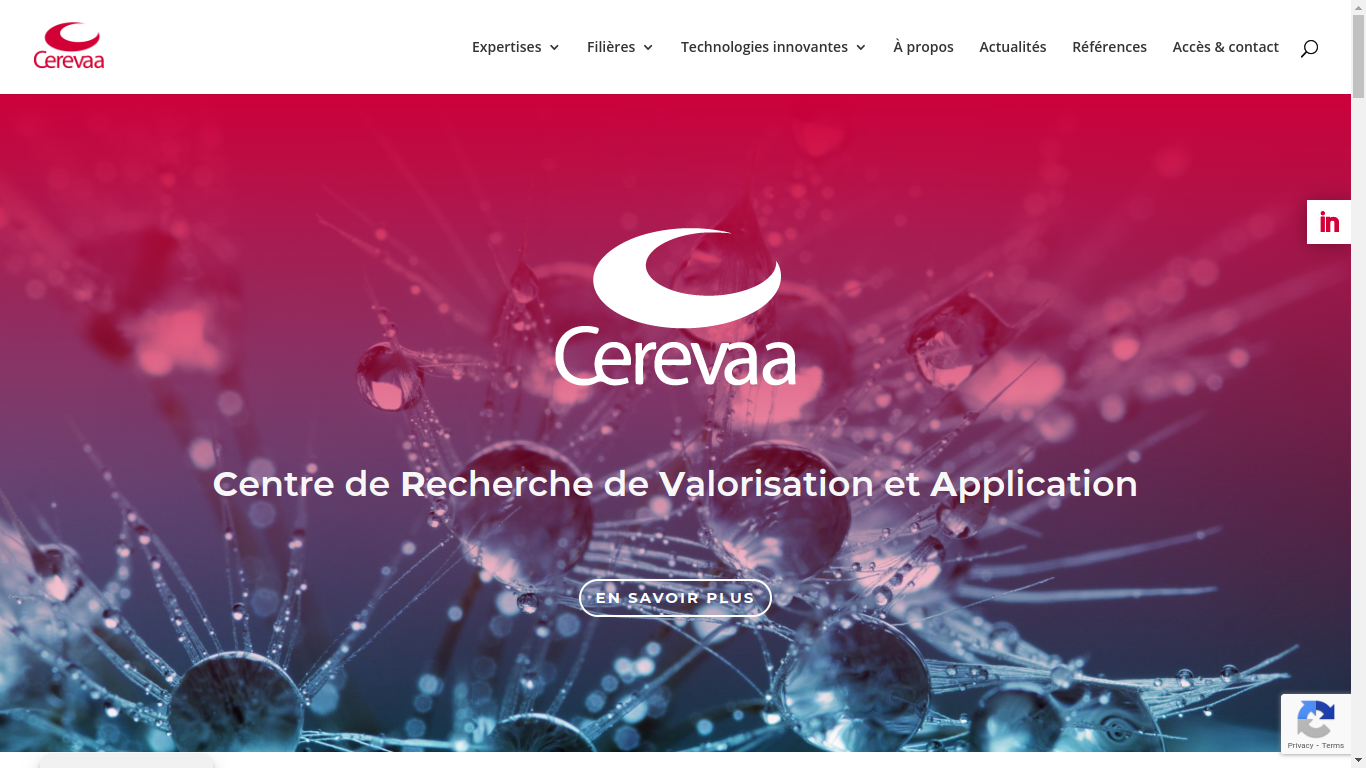
\includegraphics[width=1\textwidth]{1.png}
    \caption{Cerevaa Centre de recherche de Valorisation et Application.}
    \label{fig:mesh1}
\end{figure}
\newpage
\subsection*{CERTE Centre de recherche Et des Technologies des Eaux.}
Le CERTE est un Etablissement Public à caractère Administratif (EPA), doté de la personnalité morale et de l’autonomie financière. Il fait partie de la composante ”recherche” du Technopole de Borj Cedria (Décret de création N° 337/2005).  En 2010 (Décret n° 3483/2010), il a été transformé d’un EPA à un EPST (Etablissement Publique à caractère Scientifique et Technologique).
Dans le cadre de sa démarche de mise en place d’outils de prévention et de détection du plagiat, le Centre de Recherches et des Technologies des Eaux met à disposition de ses enseignants-chercheurs la plateforme de détection de similitudes URKUND.
Cette plateforme vous permet d'analyser des travaux rendus par les étudiants sous forme numérique, pour repérer et identifier des paragraphes similaires à des textes disponibles en ligne et dont les sources ne seraient pas citées.
l'application web Centre de recherche Et des Technologies des Eaux presente un interface pour les différents interanautes qui contient les différents section : 
\begin{itemize}
\item Domaines de travail et missions
\item Laboratoires 
\item Projets de recherches
\item Plateformes et Actualités 
\item Contact
\end{itemize}
\begin{figure}[h]
    \centering
    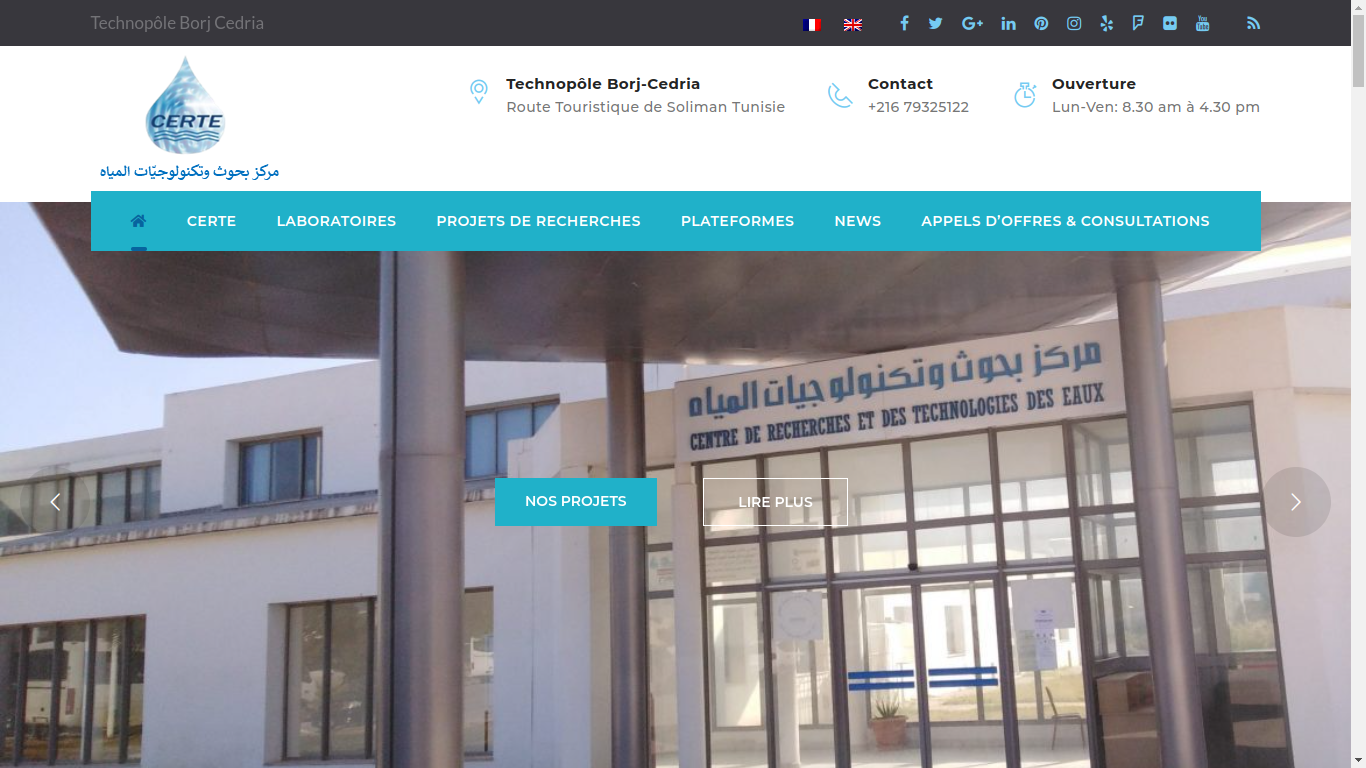
\includegraphics[width=1\textwidth]{2.png}
    \caption{Centre de recherche Et des Technologies des Eaux.}
    \label{fig:mesh1}
\end{figure}

src : https://certe.rnrt.tn/
\newpage
\subsection*{CNRSM Centre National de Recherche en sciences des matériaux.}
Le Centre National des Recherches en Sciences des Matériaux (CNRSM) est un établissement public à caractère administratif doté de la personnalité morale et de l’autonomie financière.
Son siège est fixé au technopôle de Borj Cedria. Il est crée par le décret 1599-2006 du 06/06/2006.
Le centre est placé sous la tutelle du ministère chargé de l’enseignement supérieur et de la la recherche scientifique.
Le centre est chargé d’effectuer les travaux de recherche et d’expérimentation et de développement technologique dans le domaine des sciences des matériaux et leur intégration dans le domaine économique et social.
l'application web Centre National de Recherche en sciences des matériaux presente un interface pour les différents interanautes qui contient les différents section : 
\begin{itemize}
\item Domaines de travail et missions
\item Plateformes et Actualités 
\item Contact
\end{itemize}

src : https://ucar.rnu.tn/centre-national-de-recherches-en-sciences-des-materiaux-cnrsm/
\begin{figure}[h]
    \centering
    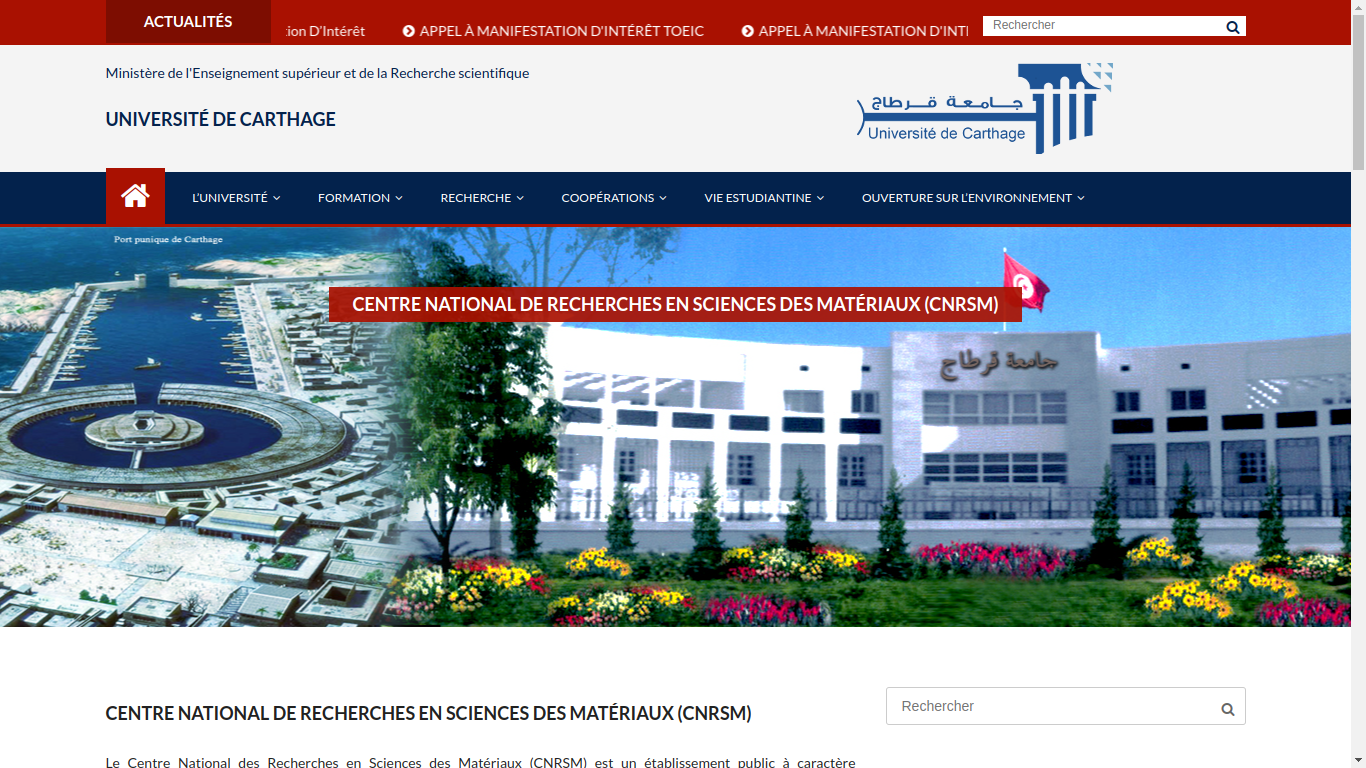
\includegraphics[width=1\textwidth]{3.png}
    \caption{CNRSM Centre National de Recherche en sciences des matériaux.}
    \label{fig:mesh1}
\end{figure}


\end{document}

